\section{TUBEPLOT Creates a Tubeplot}

\subsection{Usage}

This \verb|tubeplot| function is from the tubeplot package
written by Anders Sandberg. The simplest syntax for the
\verb|tubeplot| routine is
\begin{verbatim}
    tubeplot(x,y,z)
\end{verbatim}
plots the basic tube with radius 1, where \verb|x,y,z| are
vectors that describe the tube.  If the radius of the
tube is to be varied, use the second form
\begin{verbatim}
    tubeplot(x,y,z,r) 
\end{verbatim}
which plots the basic tube with variable radius r (either 
a vector or a scalar value).  The third form allows you
to specify the coloring using a vector of values:
\begin{verbatim}
    tubeplot(x,y,z,r,v)
\end{verbatim}
where the coloring is now dependent on the values in the 
vector \verb|v|.  If you want to create a tube plot with 
a greater degree of tangential subdivisions (i.e.,
the tube is more circular, use the form
\begin{verbatim}
    tubeplot(x,y,z,r,v,s)
\end{verbatim}
where \verb|s| is the number of tangential subdivisions (default is 6)
You can also use \verb|tubeplot| to calculate matrices to feed to \verb|mesh|
and \verb|surf|.
\begin{verbatim}
    [X,Y,Z]=tubeplot(x,y,z)
\end{verbatim}
returns \verb|N x 3| matrices suitable for mesh or surf.

Note that the tube may pinch at points where the normal and binormal 
misbehaves. It is suitable for general space curves, not ones that 
contain straight sections. Normally the tube is calculated using the
Frenet frame, making the tube minimally twisted except at inflexion points.

To deal with this problem there is an alternative frame:
\begin{verbatim}
    tubeplot(x,y,z,r,v,s,vec)
\end{verbatim}
calculates the tube by setting the normal to
the cross product of the tangent and the vector vec. If it is chosen so 
that it is always far from the tangent vector the frame will not twist unduly.
\subsection{Example}

Here is an example of a \verb|tubeplot|.
\begin{verbatim}
--> t=0:(2*pi/100):(2*pi);
--> x=cos(t*2).*(2+sin(t*3)*.3);
--> y=sin(t*2).*(2+sin(t*3)*.3);
--> z=cos(t*3)*.3;
--> tubeplot(x,y,z,0.14*sin(t*5)+.29,t,10);
\end{verbatim}


\centerline{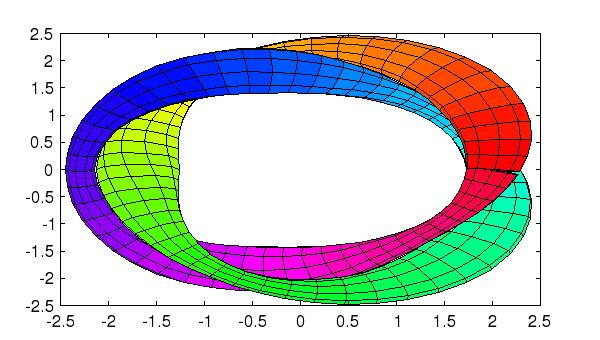
\includegraphics[width=8cm]{tubeplot1}}


 Written by Anders Sandberg, asa@nada.kth.se, 2005
 Website says the package is free for anybody to use.
 www.nada.kth.se/~asa/Ray/Tubeplot/tubeplot.html
